\documentclass{tietreport}

\usepackage{graphicx}
\usepackage{float}
\usepackage{adjustbox}
\usepackage{tikz}
\usepackage{array}
\usepackage{longtable}
\usepackage{multirow}
\usepackage{url}
\usetikzlibrary{arrows.meta,positioning,shapes.geometric,calc,fit,backgrounds}

\usepackage[
  date=year,
  style=alphabetic,
  backend=biber,
  sorting=nty,
  maxnames=5,
  minnames=3,
  maxalphanames=4,
  minalphanames=3,
  backref=true,
  doi=false,
  isbn=false,
  url=false,
  eprint=false
]{biblatex}

\begin{filecontents}{references.bib}
@misc{ultralytics2023,
  author = {Jocher, Glenn and Chaurasia, Ayush and Qiu, Jing},
  title  = {Ultralytics YOLOv8},
  year   = {2023},
  url    = {https://github.com/ultralytics/ultralytics}
}
@misc{fastapi2024,
  author = {Ram{\'i}rez, Sebasti{\'a}n},
  title  = {FastAPI},
  year   = {2024},
  url    = {https://fastapi.tiangolo.com}
}
@misc{rdd2022,
  author = {Arya, Deeksha and Solanki, Rohit and others},
  title  = {RDD2022: A Multi-National Image Dataset for Automatic Road Damage Detection},
  year   = {2022},
  url    = {https://github.com/sekilab/RoadDamageDetector}
}
@misc{sqlalchemy2024,
  author = {Bayer, Mike},
  title  = {SQLAlchemy},
  year   = {2024},
  url    = {https://www.sqlalchemy.org}
}
@misc{osm2024,
  author = {{OpenStreetMap Contributors}},
  title  = {OpenStreetMap},
  year   = {2024},
  url    = {https://www.openstreetmap.org}
}
@misc{leaflet2024,
  author = {Agafonkin, Vladimir},
  title  = {Leaflet: an open-source JavaScript library for mobile-friendly interactive maps},
  year   = {2024},
  url    = {https://leafletjs.com}
}
\end{filecontents}
\addbibresource{references.bib}

\newcommand{\screenshot}[2]{%
  \IfFileExists{#1}{%
    \includegraphics[width=0.85\textwidth]{#1}%
  }{%
    \fbox{\begin{minipage}{0.85\textwidth}\centering\vspace{1.2cm}
    \textbf{[ Screenshot to add: #2 ]}\\[0.2cm]
    \texttt{#1}\vspace{1.2cm}\end{minipage}}%
  }%
}

\TitlePageHeader{UCS503 - Software Engineering}

\ProjectTitle{CivicSight}

\ProjectSubTitle{Smart Road Damage Detection and Municipal Repair Management System}

\author{
  \texttt{1024030154} Devansh Thapar \\
  \texttt{1024030156} Laksh Garg \\
  \texttt{1024030159} Pranay Mittal
}

\TitlePageSubText{
  Group: \texttt{3C-16} B.E 3rd Year, COE
}

\AdvisorName{Ms. Paramveer Kaur}

\TitlePageFooterText{{
    \large Prototype Evaluation \\[0.2cm]
    \bfseries Computer Science and Engineering
    Department
  } \\[0.15cm]  Thapar Institute of Engineering and Technology,  Patiala
}

\tikzset{
  uc/.style={ellipse, draw, align=center, font=\scriptsize,
             inner xsep=3pt, inner ysep=1.5pt, minimum width=3.0cm,
             minimum height=0.85cm, fill=white},
  syslbl/.style={font=\small\bfseries},
  box/.style={rectangle, rounded corners, draw, align=center,
              font=\small, minimum width=3.4cm, minimum height=0.85cm,
              fill=blue!6},
  mbox/.style={rectangle, rounded corners, draw, align=center,
               font=\small, minimum width=3.0cm, minimum height=0.8cm,
               fill=green!6},
  arrow/.style={-{Stealth[length=2.5mm]}, thick},
  dasharrow/.style={-{Stealth[length=2.5mm]}, dashed, thick},
  lbl/.style={font=\scriptsize, align=center}
}
\tikzset{actorpic/.pic={
  \draw[thick] (0,0.55) circle (0.18);
  \draw[thick] (0,0.37) -- (0,-0.15);
  \draw[thick] (-0.32,0.15) -- (0.32,0.15);
  \draw[thick] (0,-0.15) -- (-0.24,-0.62);
  \draw[thick] (0,-0.15) -- (0.24,-0.62);
  \node[font=\scriptsize, align=center, anchor=north, yshift=-0.68cm] at (0,0) {#1};
}}

\begin{document}

\maketitle

\tableofcontents

\chapter{Introduction}

\section{Background and Context}

Our roads take a lot of damage every day. Heavy vehicles, rain, heat, and old construction slowly create potholes and cracks. The problem is not just the damage itself --- it is what happens after the damage appears. In most cities a citizen who spots a big pothole has to phone the municipality, maybe send a WhatsApp message, or visit an office. After that there is usually no way to know whether anyone actually saw the complaint, sent an inspector, or fixed the road. We wanted to build something that fixes this gap between ``I saw a bad road'' and ``the road is repaired and I can see the proof.''

That is where CivicSight came from. CivicSight is a web-based platform where a citizen uploads a photo of road damage, the system figures out what kind of damage it is using an AI model, the report gets a priority, a municipal officer verifies it, a maintenance crew is assigned, and finally the ticket is closed --- with every single step recorded so nothing is lost in between.


\section{Motivation}

During our Software Engineering course we had to pick a real problem and solve it the way a software company would --- week by week, with a proper proposal, diagrams, code, and testing. Road damage reporting felt like a problem we had all seen in real life, so it was easy to stay motivated. All three of us worked across the frontend, backend, and ML parts together.


\section{Problem Statement}

The main problem we are solving is the missing link between road-damage reporting and actual repair. Today, reporting is scattered (calls, messages, walk-ins), assessment is subjective (a photo alone says nothing about severity), prioritization is manual, and there is no reliable audit trail of what happened to a complaint.


\clearpage
\section{Project Objectives}

\begin{enumerate}
  \item Build a single web platform where citizens can report road damage with a photo, GPS location, and description --- and get a trackable ticket ID. \emph{(Done)}
  \item Add an AI component that automatically detects damage type (pothole, cracks) in uploaded photos and shows the result with bounding boxes. \emph{(Done)}
  \item Give municipal officers a dashboard to verify, reject, mark duplicates, and assign repairs, with every change logged in a status history. \emph{(Done)}
  \item Enforce a strict server-side lifecycle so that, for example, a report cannot be assigned before it is verified. \emph{(Done)}
  \item Keep the citizen submission fast even though ML inference takes time, by running it in the background. \emph{(Done)}
\end{enumerate}

\chapter{Methodology and Design}


\section{Overall Approach}

We followed the iterative and incremental SDLC model throughout the project. Work happened in short, repeatable iterations (one per week), and in each iteration we designed, built, and tested a small vertical increment of the system. Because increments were kept small --- reports CRUD in week 2, authentication and roles in week 3, map and ML baseline in week 4, and so on --- we got early working software, received feedback from our own demos and tests, and fixed issues before they accumulated. The backend, frontend, and ML components were developed and integrated incrementally, and every increment was validated by its own test script before we moved on. Week 7 then tied these increments together into one integrated prototype. Week 1 was just the skeleton (folders, README, health checks). Week 2 added the citizen report form and the basic database. Week 3 brought in login and roles. Week 4 made it a real end-to-end flow with maps and the first ML experiment. Week 5 added the officer verification dashboard and an improved model. Week 6 made the lifecycle strict and finalized the ML module. Week 7 glued everything together into the prototype we are submitting.

\begin{longtable}{|p{1.6cm}|p{11.6cm}|}
\hline
\textbf{Week} & \textbf{What we built} \\
\hline
1 & Monorepo skeleton (frontend, backend, ml folders), landing page, FastAPI health check, ML environment setup \\
\hline
2 & Citizen report page with photo upload, backend models and CRUD APIs, RDD2022 dataset analysis \\
\hline
3 & Registration/login with JWT, four roles (Citizen, Municipal Officer, Maintenance Staff, Admin), dataset splits and visual checks \\
\hline
4 & Interactive Leaflet map with GPS, report creation API with image storage, preprocessing pipeline, first YOLOv8n baseline \\
\hline
5 & Municipal officer dashboard (KPI cards, filters, inspection modal), verify endpoint, ML experiment 2 \\
\hline
6 & Full lifecycle state machine with strict transition rules, status history, reusable ML inference module \\
\hline
7 & End-to-end integration: async ML processing on upload, four ML states, six-checkpoint prototype audit \\
\hline
\end{longtable}


\clearpage
\section{System Architecture}

\subsection{High-Level Design}

CivicSight has three parts: the \textbf{frontend} (plain HTML/CSS/JavaScript pages in the browser), the \textbf{backend} (a FastAPI server that owns all data and business rules), and the \textbf{ML subsystem} (Python code using PyTorch and Ultralytics YOLOv8). The browser never talks directly to the ML code --- everything goes through the backend, which is important because it means we can check permissions and log every action in one place.

\begin{figure}[htbp]
\centering
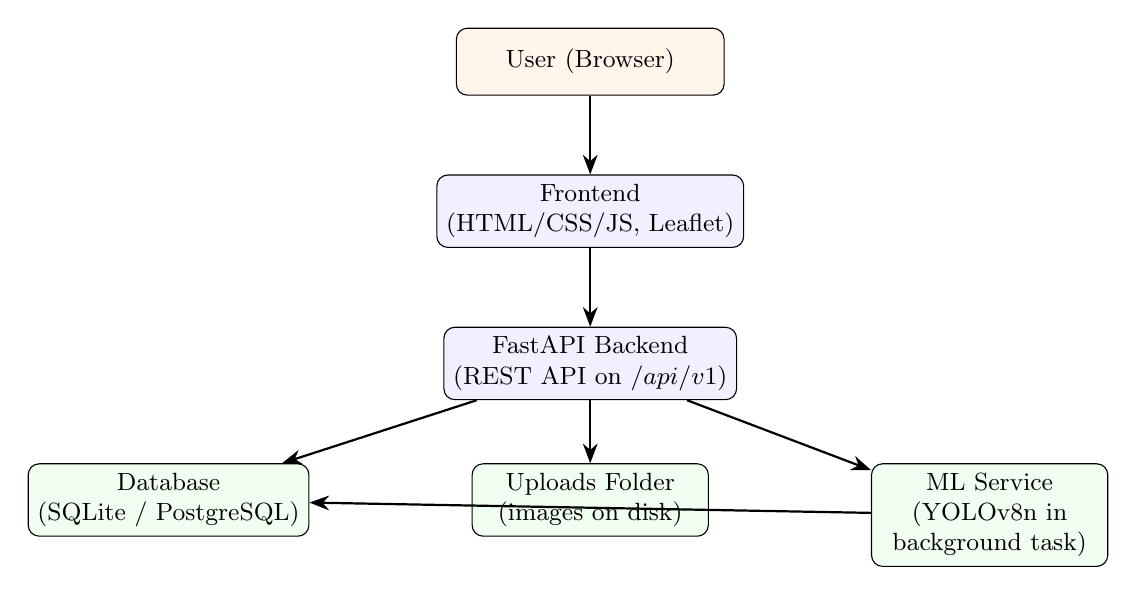
\begin{tikzpicture}[node distance=1.0cm]
  \node[box, fill=orange!8] (user) {User (Browser)};
  \node[box, below=of user] (fe) {Frontend\\(HTML/CSS/JS, Leaflet)};
  \node[box, below=of fe] (be) {FastAPI Backend\\(REST API on $/api/v1$)};
  \node[mbox, below left=0.8cm and 1.7cm of be] (db) {Database\\(SQLite / PostgreSQL)};
  \node[mbox, below=0.8cm of be] (store) {Uploads Folder\\(images on disk)};
  \node[mbox, below right=0.8cm and 1.7cm of be] (ml) {ML Service\\(YOLOv8n in\\background task)};
  \draw[arrow] (user) -- (fe);
  \draw[arrow] (fe) -- (be);
  \draw[arrow] (be) -- (db);
  \draw[arrow] (be) -- (store);
  \draw[arrow] (be) -- (ml);
  \draw[arrow] (ml) -- (db);
\end{tikzpicture}
\caption{High-level architecture of CivicSight.}
\end{figure}

\clearpage
\subsection{Request Flow when a Citizen Submits a Report}

\begin{figure}[htbp]
\centering
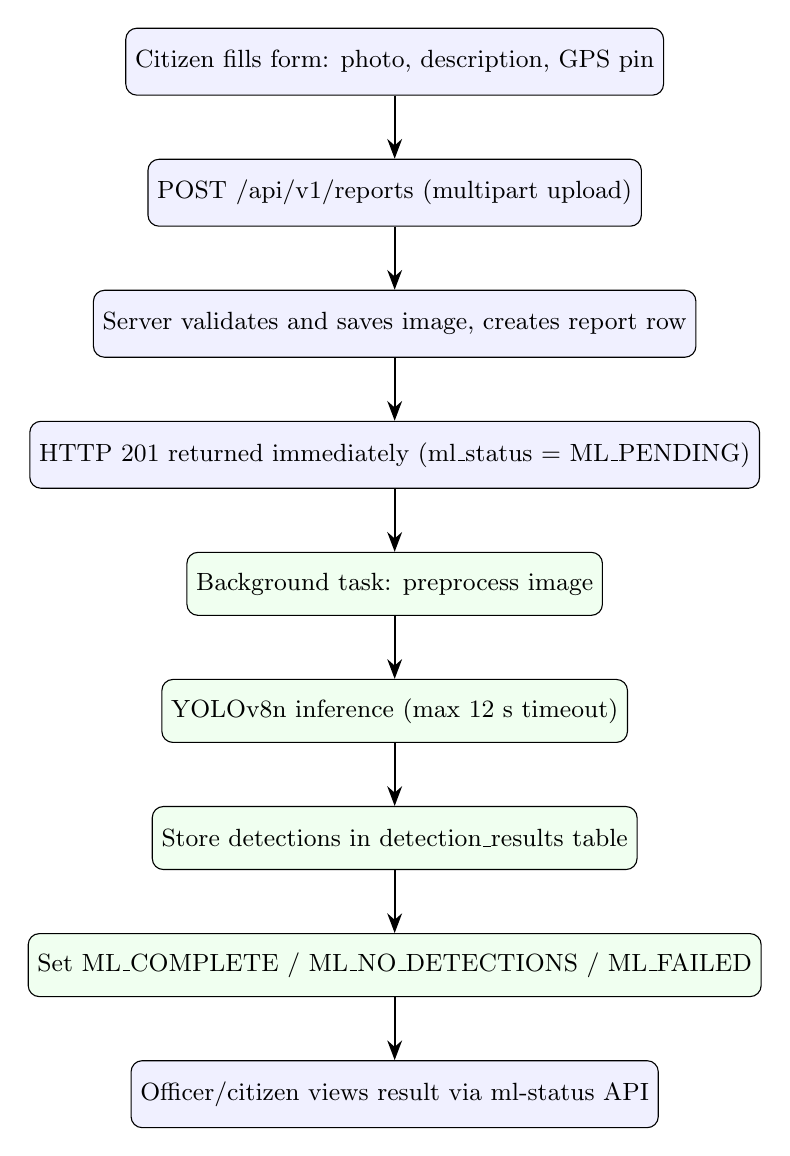
\begin{tikzpicture}[node distance=0.8cm]
  \node[box] (a) {Citizen fills form: photo, description, GPS pin};
  \node[box, below=of a] (b) {POST /api/v1/reports (multipart upload)};
  \node[box, below=of b] (c) {Server validates and saves image, creates report row};
  \node[box, below=of c] (d) {HTTP 201 returned immediately (ml\_status = ML\_PENDING)};
  \node[mbox, below=of d] (e) {Background task: preprocess image};
  \node[mbox, below=of e] (f) {YOLOv8n inference (max 12 s timeout)};
  \node[mbox, below=of f] (g) {Store detections in detection\_results table};
  \node[mbox, below=of g] (h) {Set ML\_COMPLETE / ML\_NO\_DETECTIONS / ML\_FAILED};
  \node[box, below=of h] (i) {Officer/citizen views result via ml-status API};
  \draw[arrow] (a) -- (b); \draw[arrow] (b) -- (c); \draw[arrow] (c) -- (d);
  \draw[arrow] (d) -- (e); \draw[arrow] (e) -- (f); \draw[arrow] (f) -- (g);
  \draw[arrow] (g) -- (h); \draw[arrow] (h) -- (i);
\end{tikzpicture}
\caption{Report submission and asynchronous ML processing flow.}
\end{figure}

The key design decision was that steps (e) through (h) happen \emph{after} the HTTP response. In our tests a submission returns in about 12\,ms, while the AI work takes about 40--50\,ms plus overhead --- so nothing ever feels slow for the citizen.

\clearpage
\section{Technical Stack}

\begin{itemize}
  \item \textbf{Backend:} Python 3.10+, FastAPI, SQLAlchemy 2.0, PyJWT, bcrypt, Uvicorn.
  \item \textbf{Database:} SQLite for local development; PostgreSQL for real deployment.
  \item \textbf{Frontend:} plain HTML, CSS, and JavaScript (no framework), Leaflet.js for the map, Lottie animation for the scanning effect.
  \item \textbf{ML:} PyTorch, Ultralytics YOLOv8n, dataset: RDD2022 with classes D00 (longitudinal crack), D10 (transverse crack), D20 (alligator crack), D40 (pothole).
  \item \textbf{Testing:} small Python test scripts that run against a live server.
\end{itemize}


\clearpage
\section{UML Use Case Diagram}

Figure~\ref{fig:usecase} shows everyone who uses CivicSight and what each of them can do.

\begin{figure}[htbp]
\centering
\resizebox{\textwidth}{!}{%
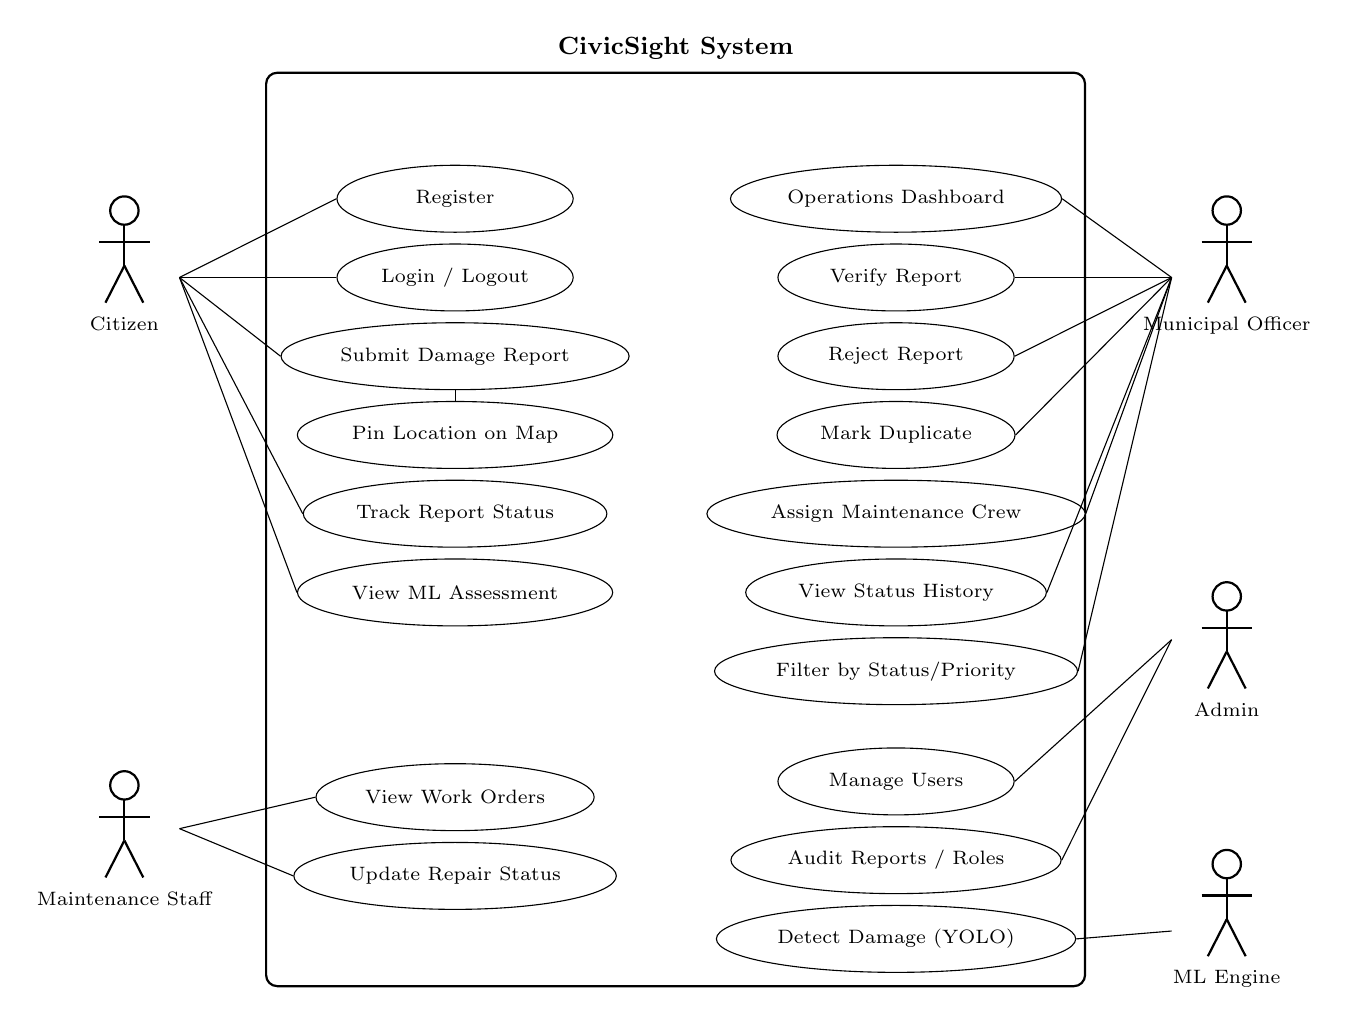
\begin{tikzpicture}[node distance=0.62cm, font=\small]
\draw[thick, rounded corners] (2.2,1.0) rectangle (12.6,-10.6);
\node[syslbl, anchor=south] at (7.4,1.05) {CivicSight System};
\pic at (0.4,-1.3) {actorpic=Citizen};
\pic at (0.4,-8.6) {actorpic=Maintenance Staff};
\pic at (14.4,-1.3) {actorpic=Municipal Officer};
\pic at (14.4,-6.2) {actorpic=Admin};
\pic at (14.4,-9.6) {actorpic=ML Engine};
\node[uc] (reg) at (4.6,-0.6) {Register};
\node[uc] (login) at (4.6,-1.6) {Login / Logout};
\node[uc] (submit) at (4.6,-2.6) {Submit Damage Report};
\node[uc] (geo) at (4.6,-3.6) {Pin Location on Map};
\node[uc] (track) at (4.6,-4.6) {Track Report Status};
\node[uc] (viewml) at (4.6,-5.6) {View ML Assessment};
\node[uc] (dash) at (10.2,-0.6) {Operations Dashboard};
\node[uc] (verify) at (10.2,-1.6) {Verify Report};
\node[uc] (reject) at (10.2,-2.6) {Reject Report};
\node[uc] (dup) at (10.2,-3.6) {Mark Duplicate};
\node[uc] (assign) at (10.2,-4.6) {Assign Maintenance Crew};
\node[uc] (hist) at (10.2,-5.6) {View Status History};
\node[uc] (filters) at (10.2,-6.6) {Filter by Status/Priority};
\node[uc] (worder) at (4.6,-8.2) {View Work Orders};
\node[uc] (updstatus) at (4.6,-9.2) {Update Repair Status};
\node[uc] (users) at (10.2,-8.0) {Manage Users};
\node[uc] (audit) at (10.2,-9.0) {Audit Reports / Roles};
\node[uc] (detect) at (10.2,-10.0) {Detect Damage (YOLO)};
\draw (1.1,-1.6) -- (reg.west);
\draw (1.1,-1.6) -- (login.west);
\draw (1.1,-1.6) -- (submit.west);
\draw (1.1,-1.6) -- (track.west);
\draw (1.1,-1.6) -- (viewml.west);
\draw (submit.south) -- (geo.north);
\draw (1.1,-8.6) -- (worder.west);
\draw (1.1,-8.6) -- (updstatus.west);
\draw (13.7,-1.6) -- (dash.east);
\draw (13.7,-1.6) -- (verify.east);
\draw (13.7,-1.6) -- (reject.east);
\draw (13.7,-1.6) -- (dup.east);
\draw (13.7,-1.6) -- (assign.east);
\draw (13.7,-1.6) -- (hist.east);
\draw (13.7,-1.6) -- (filters.east);
\draw (13.7,-6.2) -- (users.east);
\draw (13.7,-6.2) -- (audit.east);
\draw (13.7,-9.9) -- (detect.east);
\end{tikzpicture}%
}
\caption{Use case diagram covering all CivicSight functionalities.}
\label{fig:usecase}
\end{figure}


\clearpage
\section{Lifecycle State Machine}

A report in CivicSight can be in these states: \texttt{submitted}, \texttt{pending\_verification}, \texttt{verified}, \texttt{rejected}, \texttt{duplicate}, \texttt{assigned}, \texttt{under\_repair}, \texttt{repaired}, \texttt{closed}. The important part is that the server itself decides which moves are legal --- the frontend cannot cheat the workflow.

\begin{figure}[htbp]
\centering
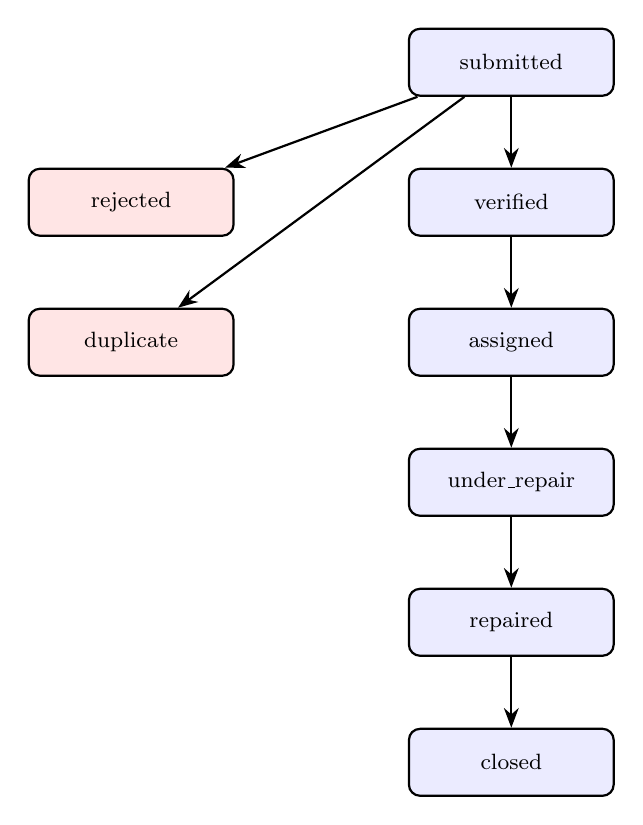
\begin{tikzpicture}[node distance=0.9cm and 1.8cm,
  lnb/.style={rectangle, rounded corners, draw, thick, align=center,
              font=\footnotesize, minimum width=2.6cm, minimum height=0.85cm,
              fill=blue!8},
  snb/.style={rectangle, rounded corners, draw, thick, align=center,
              font=\footnotesize, minimum width=2.6cm, minimum height=0.85cm,
              fill=red!10}]
  \node[lnb] (s) {submitted};
  \node[lnb, below=0.9cm of s] (v) {verified};
  \node[lnb, below=0.9cm of v] (a) {assigned};
  \node[lnb, below=0.9cm of a] (u) {under\_repair};
  \node[lnb, below=0.9cm of u] (r) {repaired};
  \node[lnb, below=0.9cm of r] (c) {closed};
  \node[snb, left=2.2cm of v] (rej) {rejected};
  \node[snb, left=2.2cm of a] (dup) {duplicate};
  \draw[arrow] (s) -- (v);
  \draw[arrow] (v) -- (a);
  \draw[arrow] (a) -- (u);
  \draw[arrow] (u) -- (r);
  \draw[arrow] (r) -- (c);
  \draw[arrow] (s) -- (rej);
  \draw[arrow] (s) -- (dup);
\end{tikzpicture}
\caption{Legal lifecycle transitions of a report (simplified).}
\end{figure}

Some rules the server enforces: a report cannot be assigned before it is verified; once assigned it cannot be rejected; a closed or repaired report cannot be verified again. Breaking the rules returns an HTTP 400 error. Every allowed change is written into a \texttt{report\_status\_history} table, which gives the officer a full audit trail.


\clearpage
\section{ML Pipeline Design}

\begin{figure}[htbp]
\centering
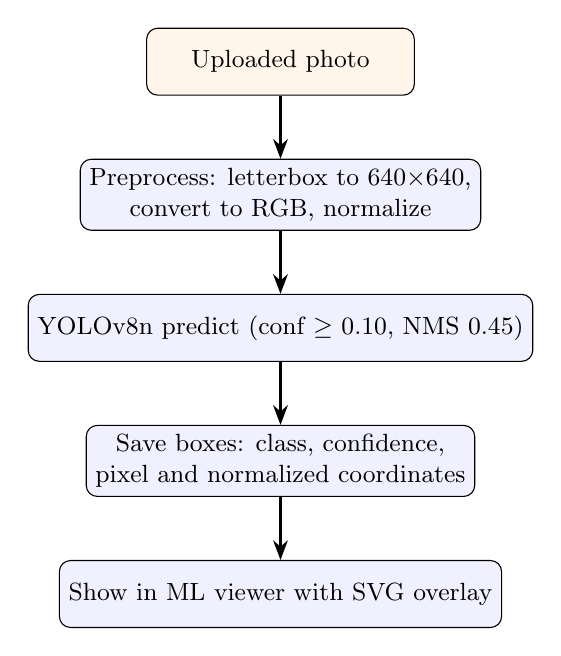
\begin{tikzpicture}[node distance=0.8cm]
  \node[box, fill=orange!8] (img) {Uploaded photo};
  \node[box, below=of img] (pp) {Preprocess: letterbox to 640$\times$640,\\convert to RGB, normalize};
  \node[box, below=of pp] (yolo) {YOLOv8n predict (conf $\geq$ 0.10, NMS 0.45)};
  \node[box, below=of yolo] (db2) {Save boxes: class, confidence,\\pixel and normalized coordinates};
  \node[box, below=of db2] (view) {Show in ML viewer with SVG overlay};
  \draw[arrow] (img) -- (pp); \draw[arrow] (pp) -- (yolo);
  \draw[arrow] (yolo) -- (db2); \draw[arrow] (db2) -- (view);
\end{tikzpicture}
\caption{Machine learning pipeline inside the backend background task.}
\end{figure}

We used the RDD2022 dataset, split as 26{,}869 training, 5{,}758 validation, and 5{,}758 test images. We trained two experiments. Experiment 1 (Week 4) was very weak (mAP@0.5 of 0.0335). Experiment 2 (Week 5) fixed this by lowering the input size to 512, training for 3 epochs, and using cosine learning-rate scheduling --- precision jumped from 0.0041 to 0.6541 and mAP@0.5 went up by about 251\%.

\chapter{Implementation}

\section{Backend}

The backend is built with FastAPI. The main file \texttt{app/main.py} starts the app, enables CORS (so the frontend on another port can call it), mounts the \texttt{/uploads} folder for serving images, and registers the API routers. All database models live in \texttt{app/models/models.py}.

\subsection{Authentication and Roles}

Registration stores a bcrypt hash of the password --- never the plain password. Login checks the password against the hash and returns a JWT token that the frontend keeps in \texttt{localStorage}. Two reusable helper functions protect endpoints: one that checks ``is this a logged-in user'', and one that checks the role (e.g.~only Municipal Officer and Admin). We tested that a citizen token gets 403 Forbidden on officer endpoints.

\subsection{Reports API}

\begin{longtable}{|l|p{8.4cm}|}
\hline
\textbf{Endpoint} & \textbf{Purpose} \\
\hline
POST \texttt{/api/v1/auth/register} & Create a new account \\
\hline
POST \texttt{/api/v1/auth/login} & Get a JWT token \\
\hline
POST \texttt{/api/v1/reports} & Submit a report with photo and location \\
\hline
GET \texttt{/api/v1/reports} & List reports, filter by status/priority \\
\hline
GET \texttt{/api/v1/reports/\{id\}/ml-status} & Check ML processing state \\
\hline
PATCH \texttt{/api/v1/reports/\{id\}/verify} & Officer verifies the report \\
\hline
PATCH \texttt{/api/v1/reports/\{id\}/assign} & Give to a maintenance crew \\
\hline
GET \texttt{/api/v1/reports/\{id\}/history} & Full audit timeline \\
\hline
\end{longtable}

\subsection{ML Service}

The file \texttt{app/services/ml\_service.py} runs inside a background task. It takes the saved image, runs preprocessing and inference with a timeout, writes one row per detected defect into \texttt{detection\_results}, and updates the report's \texttt{ml\_status}. Because the UI has four possible ML states (pending, complete, no detections, failed), the frontend always knows exactly what to show --- it never displays a confusing blank box.


\section{Frontend}

The frontend has no framework --- just static pages. We keep it simple so that hosting is trivial (any static server works).

\begin{figure}[htbp]
\centering
\screenshot{screenshots/report.jpeg}{Citizen report page}
\caption{Damage report page: drag-and-drop photo, description, and Leaflet map with GPS.}
\end{figure}

\begin{figure}[htbp]
\centering
\screenshot{screenshots/dashboard.jpeg}{Officer dashboard}
\caption{Municipal officer dashboard with KPI cards, filters, and live report table.}
\end{figure}

\begin{figure}[htbp]
\centering
\screenshot{screenshots/mlviewer.jpeg}{ML detection viewer}
\caption{Inspection modal showing the AI detection with bounding boxes and the audit timeline.}
\end{figure}


\clearpage
\section{ML Subsystem}

We keep all ML code inside the \texttt{ml/} folder: \texttt{data.yaml} points to the dataset, \texttt{src/preprocess.py} contains the reusable preprocessing, \texttt{src/inference.py} is the reusable inference function used by the backend, and \texttt{scripts/} has the scripts for training, testing, and dataset visualization. The weights used in production are from experiment 2, saved at \texttt{ml/runs/detect/experiment2\_week5/weights/best.pt}.

\begin{figure}[htbp]
\centering
\screenshot{screenshots/dataset_distribution.jpeg}{Class distribution chart}
\caption{Distribution of classes in the RDD2022 training split.}
\end{figure}

\begin{figure}[htbp]
\centering
\screenshot{screenshots/rd2022.png}{ML detection result}
\caption{Sample YOLOv8n detection output with bounding boxes on a road image.}
\end{figure}

\chapter{Results and Testing}

\section{Testing Strategy}

We did not follow heavy formal testing --- we kept it practical:

\begin{itemize}
  \item Small Python test scripts for authentication (register, login, token checks, RBAC 403s).
  \item Test scripts for the reports API: creating reports, filtering, verification rules.
  \item Test scripts for the lifecycle: valid path works, illegal paths return 400, history rows appear.
  \item A six-checkpoint end-to-end script (Week 7) that runs against a live server and a real database.
\end{itemize}

\section{Prototype Test Results}

\begin{longtable}{|c|p{6.2cm}|p{5.0cm}|c|}
\hline
\textbf{\#} & \textbf{What we tested} & \textbf{What happened} & \textbf{Result} \\
\hline
1 & Upload a real pothole photo & Report created in 11.6\,ms, ml\_status = ML\_PENDING & Pass \\
\hline
2 & Wait for ML to finish & ML\_COMPLETE, D40 pothole detected, confidence 0.335 & Pass \\
\hline
3 & Upload a clean road photo & ML\_NO\_DETECTIONS, no error & Pass \\
\hline
4 & Upload a corrupted image & ML\_FAILED, but the report itself stayed valid & Pass \\
\hline
5 & Officer verifies the report & Status changed to verified; AI section stayed separate & Pass \\
\hline
6 & Restart the server & Same detections still returned by the API & Pass \\
\hline
\end{longtable}


\clearpage
\section{ML Results}

\begin{table}[H]
\centering
\begin{tabular}{|l|r|r|r|}
\hline
\textbf{Metric} & \textbf{Exp 1} & \textbf{Exp 2} & \textbf{Change} \\
\hline
Precision & 0.0041 & 0.6541 & +0.65 \\
\hline
Recall & 0.5024 & 0.1254 & $-$0.377 \\
\hline
mAP@0.5 & 0.0335 & 0.1176 & +251\% \\
\hline
mAP@0.5:0.95 & 0.0114 & 0.0530 & +365\% \\
\hline
\end{tabular}
\caption{YOLO experiment comparison.}
\end{table}

Potholes (D40) are the easiest class for our model; alligator cracks (D20) are still very hard and that is our biggest weakness. Latency on a normal laptop CPU: preprocessing about 8\,ms, inference about 40\,ms, total pipeline under 50\,ms.


\section{Discussion}

The prototype does what we aimed for: a complete path from a citizen complaint to a closed ticket, with an AI assist in the middle. Two honest observations: (1) the model's recall is low --- it prefers to stay quiet rather than shout wrong answers, which we think is the right trade-off for a first version; (2) the async ML design was the single most important decision in the project, because it made the whole system feel fast regardless of model speed.

\chapter{Conclusion and Future Work}


\section{Conclusion}

In seven weeks we took CivicSight from an empty folder to a working prototype. A citizen can register, report a road problem with a photo and a map pin, and watch the ticket get detected, verified, and repaired --- while the municipality gets a dashboard with real numbers and a full audit trail. The AI part is honest about its limits: it shows its confidence and never pretends to be the final word.


\section{Future Work}

\begin{itemize}
  \item Proper notifications (email/SMS) when a ticket changes status.
  \item Improve D20 alligator-crack detection with more data and longer training.
  \item A map view showing all reports together, so hotspots are visible.
  \item Deploy on a real server with PostgreSQL and HTTPS.
  \item Mobile-friendly PWA so citizens can report directly from the spot.
\end{itemize}


\section{Lessons Learned}

Keeping the frontend, backend, and ML in one monorepo saved us a lot of confusion. Writing small test scripts early (instead of testing only at the end) caught many bugs --- especially illegal lifecycle moves. And planning the async ML design on paper first made Week 7 much less painful than it would have been otherwise.

\printbibliography[heading=bibintoc]

\end{document}
